\documentclass{beamer}
\usetheme{Darmstadt}
\definecolor{UBCblue}{rgb}{0.04706, 0.13725, 0.26667}
\usecolortheme[named=UBCblue]{structure}
% \setbeamertemplate{navigation symbols}{}
\setbeamertemplate{footline}[frame number]
\setbeamercolor{background canvas}{bg=}

% \usepackage[backend=bibtex,style=authoryear]{biblatex}
% \addbibresource{ref.bib}
\usepackage{babel}
\usepackage[%
style=authortitle, % numeric, alphabetic, authoryear, ect.
sorting=nty,
isbn=false,
abbreviate = false,
backend=bibtex,]{biblatex}
\addbibresource{ref.bib}

\usepackage{pgf}
\usepackage{epsfig}
\usepackage{epstopdf}
\usepackage{graphicx}
\usepackage{url}
\usepackage{listings}
\usepackage{xcolor}
\usepackage{xparse}
\usepackage{verbatim}
\usepackage{algorithm}
\usepackage{algpseudocode}
\usepackage{caption}

\captionsetup[figure]{font=footnotesize}
\captionsetup{justification=centering}

\usepackage[utf8]{inputenc}
\usepackage{polski}

\newcommand{\IR}{\bbold R}
\def\Rset{\mathbb{R}}
\def\Zset{\mathbb{Z}}
\newcommand{\refbr}[1]{(\ref{#1})}
\newcommand{\beq}{\begin{equation}}
\newcommand{\eeq}{\end{equation}}
\newcommand{\und}[1]{\underline{#1}}

\hypersetup{
   pdftitle={Julia Jodczyk, SDM 2024},
   pdfauthor={Julia Jodczyk, II},
   pdfborder={0 0 0}
}

\title[ \insertframenumber/\inserttotalframenumber]{Optymalizacja ścieżek reprezentacji przestrzeni na potrzebę obsługi efektów lokalnych w symulacji transportu światła}
\author[Julia Jodczyk]{\textbf{Julia Jodczyk}}
\institute{Instytut Informatyki \\
dr inż. Łukasz Dąbała}

\date{\tiny{\emph{6 listopada 2024
}}}

\begin{document}

\frame{\titlepage}

\frame{\tableofcontents\frametitle{Plan prezentacji}}

\section{Śledzenie promieni}

\begin{frame}
\frametitle{Fotorealiztyczny rendering}
\begin{itemize}
    \item Rendering to proces generacji obrazu z modelu za pomocą programu komputerowego.
    \item Celem fotorealistycznego renderingu jest stworzenie obrazu, który jest nie do odróżnienia od zdjęcia.
\end{itemize}
\end{frame}

\begin{frame}
\frametitle{Śledzenie promieni \it{ang. Ray tracing}}
\begin{itemize}
    \item Aby generować realistyczne obrazy, potrzebna jest jak najlepsza symulacja fizyki światła i jego interakcji z materią.
    \item Wykorzystuje się do niej model światła w postaci cząsteczki poruszające się po promieniach.
    \item Algorytm śledzenia promieni opiera się na podążaniu ścieżką promienia światła przez scenę.
\end{itemize}
\end{frame}

\begin{frame}
\frametitle{Algorytm}
\begin{enumerate}
    \item Z kamery w kierunku piksela prowadzony jest promień.
    \item Wyszukiwany jest najbliższy punkt przecięcia z obiektami w scenie.
    \item Z tego punktu promienie prowadzone są do każdego źródła światła, w celu wyznaczania jasność w tym punkcie.
    \item Jeśli punkt przecięcia należy do obiektu odbijającego światło lub przeźroczystego to wysyłane są promienie wtórne.
\end{enumerate}
\end{frame}


\section{Równanie renderingu}
\begin{frame}
\frametitle{Śledzenie ścieżek \it{(ang. Path tracing)}}
\begin{itemize}
    \item Bardziej zaawansowana forma śledzenia promieni.
    \item Przy każdym uderzeniu promienia w powierzchnię jest on probabilistycznie rozpraszany w losowym kierunku.
    \item Pozwala to na symulację złożonych interakcji światła, takich jak oświetlenie pośrednie, miękkie cienie i kaustyki.
\end{itemize}
\end{frame}

\begin{frame}{}
    \begin{figure}
        \centering
        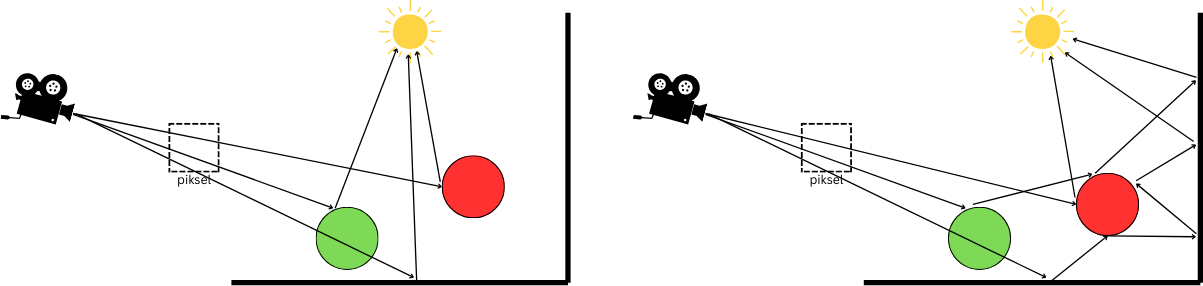
\includegraphics[width=1\linewidth]{img/path_vs_ray.png}
        \caption{Porównanie śledzenia promieni (na lewo) i śledzenia ścieżek (na prawo)}
        \label{fig:enter-label}
    \end{figure}
\end{frame}

\begin{frame}{Radiancja}
    \begin{itemize}
        \item Światło, które dociera do kamery z danego punktu, jest sumą światła emitowanego przez obiekt i światła przez niego odbitego.
        \item Ta idea sformalizowana jest przez równanie renderingu, które mierzy światło w odniesieniu do radiancji.
        \item Radiancja jest jednostką radiometryczną wyrażającą strumień promieniowania na jednostkę powierzchni z kąta bryłowego.
        \item Mówi nam, ile światła dociera do naszego oka (lub kamery) z danego miejsca i kierunku, określając, jak jasne i szczegółowe wydają się rzeczy.
        \item Radiancja pozostaje stała wzdłuż promienia światła.
    \end{itemize}
\end{frame}

\begin{frame}{Równianie renderingu}
$$ L_o(x, \omega_o) = L_e(x, \omega_o) + L_r(x, \omega_o) $$
gdzie
\begin{itemize}
    \item $L_e$ to światło emitowane przez obiekt,
    \item $L_r$ to światło odbite.
\end{itemize}
\end{frame}

\begin{frame}{BRDF \it{(Bidirectional Reflectance Distribution Function)}}
    \begin{itemize}
        \item Funkcja opisująca, jak powierzchnia obiektu odbija światło.
        \item Zależy od kierunku, z którego pada światło oraz kierunku, w którym światło jest odbijane.
    \end{itemize}
$$ f_r(x, \omega_i \rightarrow \omega_o) $$
\begin{figure}
    \centering
    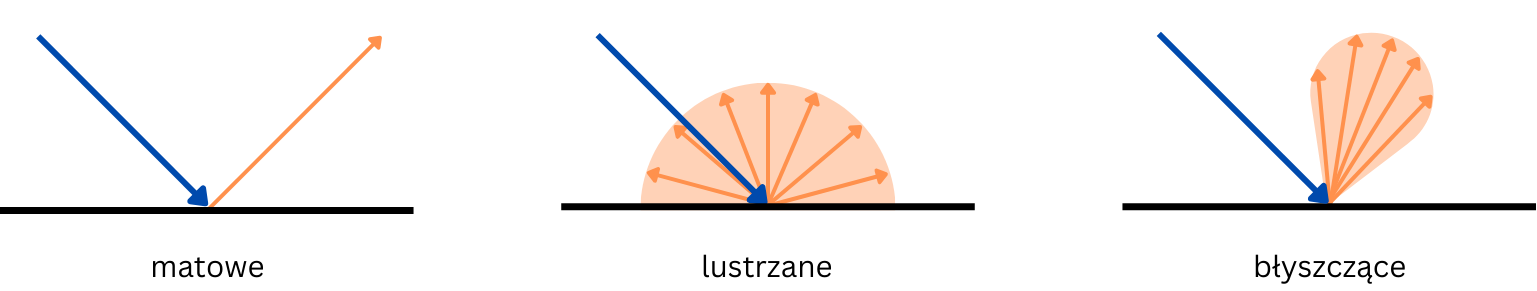
\includegraphics[width=1\linewidth]{img/surfaces.png}
    \label{fig:enter-label}
\end{figure}
\end{frame}

\begin{frame}{Światło odbite}
    $$ L_r(x, \omega_o) = \int_{\Omega}f_r(x, \omega_i \rightarrow \omega_o)L_i(x, \omega_i)cos\delta d\omega $$
gdzie
\begin{itemize}
    \item $\Omega$ to półkula wszystkich kierunków przychodzących do punktu,
    \item $L_i(x, \omega_i)$ to światło przychodzące z kierunku $\omega_i$,
    \item $cos\delta$ to tłumienie światła
\end{itemize}
\end{frame}

\section{Path guiding}

\begin{frame}{Monte Carlo}
    \begin{itemize}
        \item Równanie renderingu wymaga uwzględnienia nieskończonej liczby możliwych interakcji światła z powierzchniami sceny.
        \item Rozwiązanie tego równania nie jest możliwe, z wyjątkiem najprostrzych scen.
        \item W praktyce przybliża się je przy pomocy Monte Carlo.
    \end{itemize}
\end{frame}

\begin{frame}{Monte Carlo}
$$L_o(x, \omega_o) \approx L_e(x, \omega_o) + \frac{1}{N} \sum_{i=1}^{N} \frac{f_r(x, \omega_i, \omega_o) \, L_i(x, \omega_i) \, cos\delta}{p(\omega_i)}
$$
gdzie
\begin{itemize}
    \item N to liczba próbek,
    \item $p(\omega_i)$ to funkcja gęstości prawdopodobieństwa (PDF, \it{ang. Probability Density Function}) \normalfont wybrania kierunku $\omega_i$
    \item ułamek $\frac{f_r(x, \omega_i, \omega_o) \, L_i(x, \omega_i) \, cos\delta}{p(\omega_i)}$ waży każdą próbkę w oparciu o jej udział w radiancji.
\end{itemize}
\end{frame}

\begin{frame}{Path guiding}
    \begin{itemize}
        \item Estymacja MC zbiega do pożądanej całki wraz ze wzrostem próbek.
        \item Szybkość zbieżności można znacznie poprawić poprzez umiejętny dobór PDF.
        \item Path guiding optymalizuje path tracing poprzez inteligentne kierowanie ścieżek promieni w stronę obszarów sceny, gdzie mają one większe szanse na istotne interakcje świetlne.
        \item Podczas renderowania system uczy się, które obszary sceny emitują lub odbijają więcej światła poprzez analizowanie wcześniej obliczonych próbek.
    \end{itemize}
\end{frame}

\begin{frame}
\begin{figure}
    \centering
    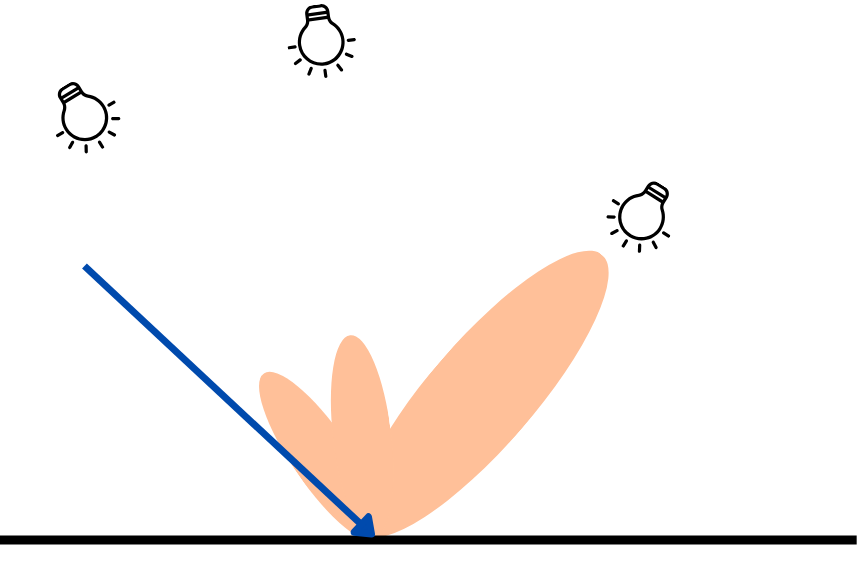
\includegraphics[width=0.9\linewidth]{img/PDF.png}
    \caption{Przykładowy rozkład PDF}
    \label{fig:enter-label}
\end{figure}
\end{frame}

\section{GMM}
\begin{frame}{Mieszanina rozkładów Gaussa}
\begin{itemize}
    \item Jednym ze sposobów uczenia się rozkładu światła przez system jest wykorzystanie mieszaniny rozkładów Gaussa.
    \item Jest to model probabilistyczny, w którym rozkład danych reprezentuje się za pomocą wielu rozkładów Gaussowskich.
    \item Funkcja gęstości prawdopodobieństwa jest zdefiniowana jako:
$$p(x) = \sum_{k=1}^{K} \pi_k \, \mathcal{N}(x \mid \mu_k, \Sigma_k)$$
\end{itemize}

gdzie
\begin{itemize}
    \item K to liczba rozkładów,
    \item $\pi_k$ to waga rozkładu,
    \item $\mathcal{N}(x \mid \mu_k, \Sigma_k)$ to rozkład Gaussa o średniej $\mu_k$ i odchyleniu standardowym $\Sigma_k$
\end{itemize}
\end{frame}

\begin{frame}{Algorytm EM}
\begin{itemize}
    \item Parametry mieszaniny są szacowane przy użyciu algorytmu EM (\it{ang. Expectation-Maximization}).
    \item \normalfont Algorytm składa się z dwóch kroków wykonywanych naprzemiennie aż do uzyskania zbieżności.
    \begin{itemize}
        \item Krok E: Obliczenie prawdopodobieństwa, że każdy punkt danych należy do każdego z rozkładów Gaussa biorąc pod uwagę bieżące oszacowania parametrów.
        \item Krok M: Aktualizacja parametrów w calu maksymalizowania prawdopodobieństwa zaobserwowanych danych przy użyciu prawdopodobieństw z kroku E.
    \end{itemize}
\end{itemize}
\end{frame}

\section{GMM w path guidingu}
\begin{frame}{Zastosowanie w path guidingu}
    \begin{itemize}
        \item Z każdą iteracją renderingu, mieszanina dostosowuje się do nowych ścieżek światła i obserwowanych kierunków, stale udoskonalając swój model.
        \item Dzięki temu można obniżyć liczbę próbek i skrócić czas potrzebny do uzyskania niezaszumionego obrazu.
    \end{itemize}
\end{frame}

\begin{frame}{Przykład zastosowania}
\begin{figure}
    \centering
    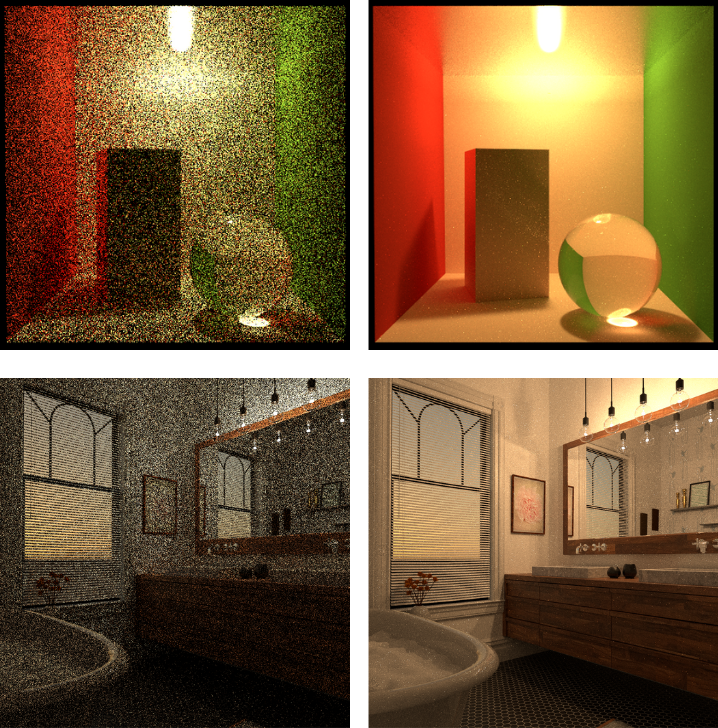
\includegraphics[width=0.42\linewidth]{img/ruppert_comparison.png}
    \caption{Porównanie standardowego śledzenia ścieżek (po lewej) i path guidingu z wykorzystaniem mieszanin rozkładów (po prawej).\footcite{PMM}}
    \label{fig:enter-label}
\end{figure}

\end{frame}

\begin{frame}{}
    \begin{figure}
        \centering
        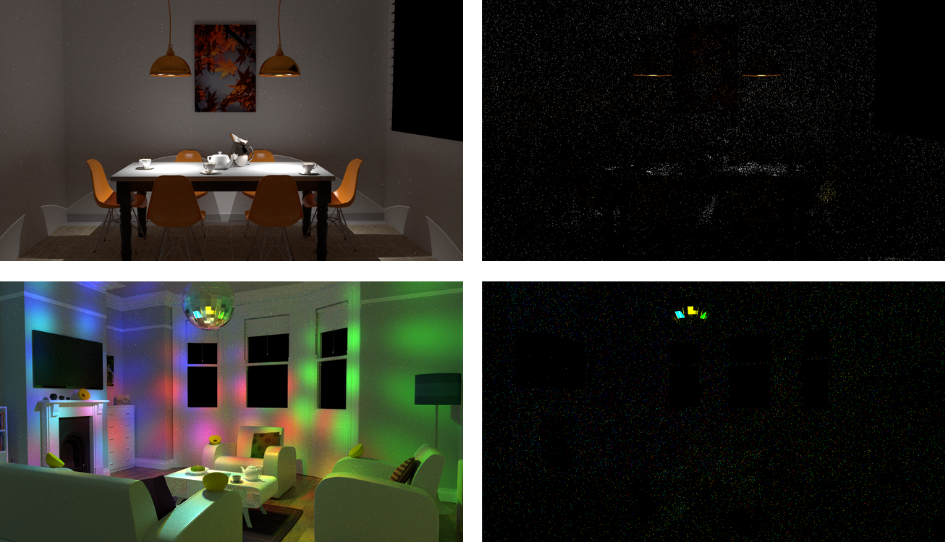
\includegraphics[width=0.8\linewidth]{img/ruppert_focal_bad.png}
        \caption{Obraz referencyjny (po lewej) i wyniki zastosowania path guidingu z wykorzystaniem mieszanin rozkładów (po prawej).\footcite{Focal_Guiding}}
        \label{fig:enter-label}
    \end{figure}
\end{frame}

\section{Efekty ogniskowe}
\begin{frame}{Efekty ogniskowe}
    \begin{itemize}
        \item Ogniska powstają, gdy wiele ścieżek światła z różnych kierunków zbiega się w małym obszarze.
        \item Ogniskami mogą być:
        \begin{itemize}
            \item bezpośrednie i pośrednie źródła światła (takie jak kaustyki i plamy),
            \item wąskie szczeliny,
            \item ogniska pozorne.
        \end{itemize}
    \end{itemize}
\end{frame}

\begin{frame}{Trudności w renderowaniu scen z ogniskami}
    \begin{itemize}
        \item Niektóre ogniska mogą pojawiać się wolnej przestrzeni, a nie na powierzchni.
        \item Niektóre typy ognisk na powierzchni są trudne do próbkowania (okluzyjne ogniska i ogniska pozorne).
    \end{itemize}
    \begin{figure}
        \centering
        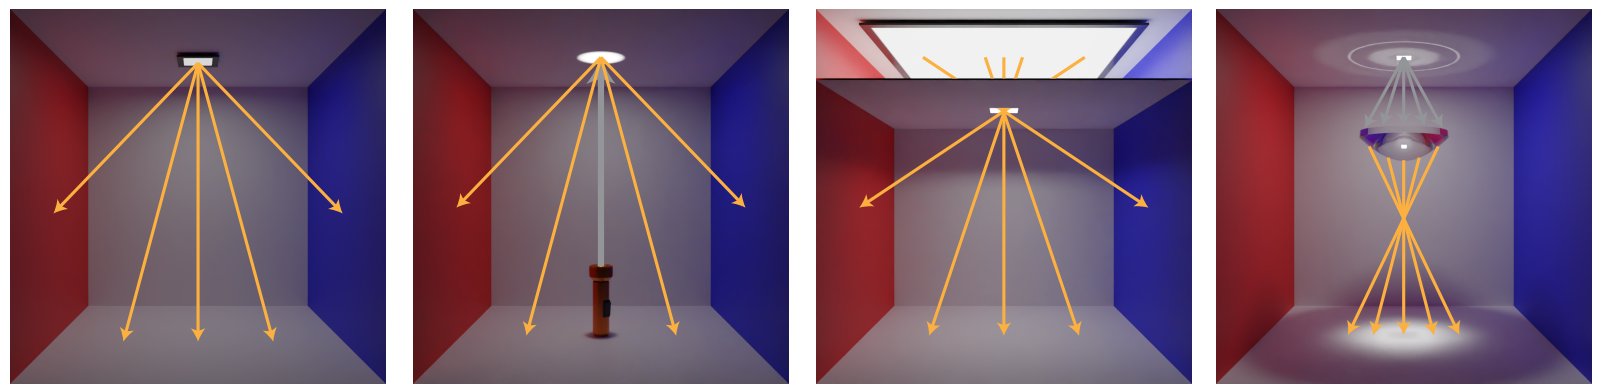
\includegraphics[width=0.8\linewidth]{img/focal_effects.png}
        \caption{Rodzaje ognisk\footcite{Focal_Guiding}}
        \label{fig:enter-label}
    \end{figure}
\end{frame}
%

\begin{frame}{Przestrzenna funkcja gęstości próbkowania}
Rath i in.\footcite{Focal_Guiding} zaproponowali nowatorską metodę path guidingu przeznaczoną do obsługi efektów ogniskowych.
    \begin{itemize}
        \item Alternatywa do bezpośredniego uczenia się kierunkowego rozkładu lokalnego.
        \item Uczenie się globalnego rozkładu ognisk w przestrzeni.
        \item Próbkowanie punktów i wyliczanie z nich następnego kierunku ścieżki:
        $$ w_o = \frac{y-x}{||y-x||} $$
    \end{itemize}
\end{frame}

\begin{frame}{Rozkład kierunkowy a przestrzenny}
    \begin{figure}
        \centering
        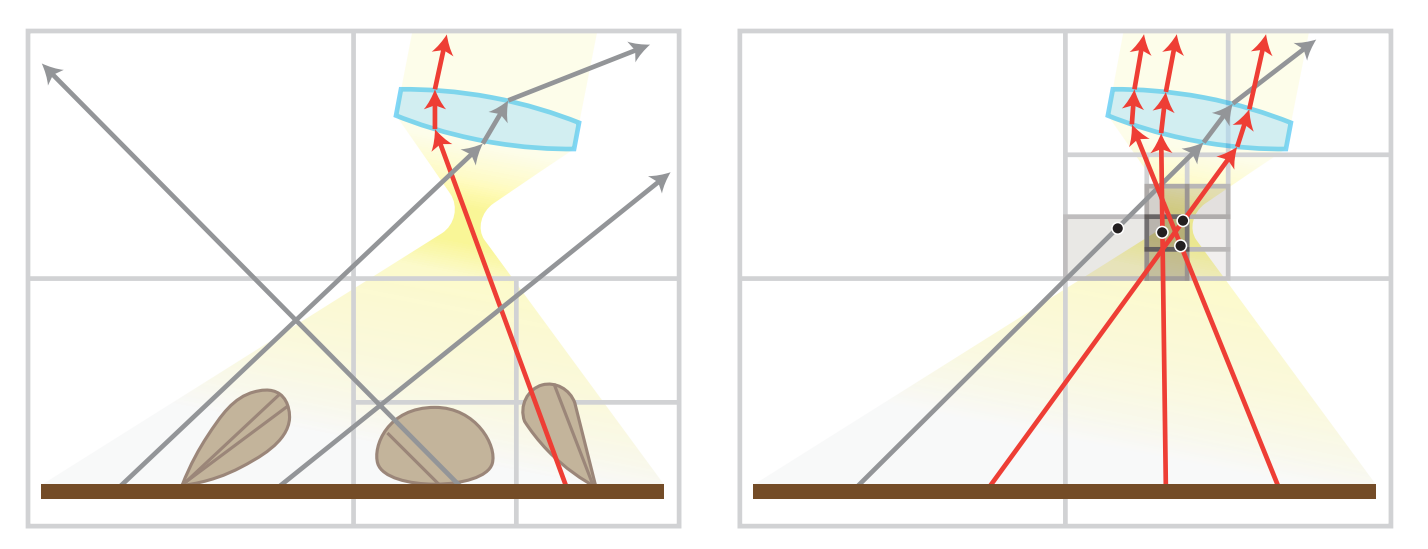
\includegraphics[width=1\linewidth]{img/directional_vs_spatial.png}
        \caption{Porównanie rozkładu kierunkowego i przestrzennego\footcite{Focal_Guiding}}
        \label{fig:enter-label}
    \end{figure}
\end{frame}

\begin{frame}{Jak znaleźć punkty ogniskowe w przestrzeni}
    \begin{itemize}
        \item Ogniska to takie punkty, w których przecina się wiele ścieżek.
        \item Przecięcie ścieżek to przecięcie prostych, na których leżą (nawet jeśli takie przecięcie znajduje się przed początkiem promienia lub za przecięciem z powierzchnią).
        \item Jeśli dla każdego punktu w scenie zliczymy wkład wszystkich ścieżek, które przez niego przechodzą, to otrzymamy funkcję, która będzie osiągała maksima w ogniskach.
    \end{itemize}
\end{frame}

\begin{frame}{Funkcja wkładu punktu}
    $$\mathcal{F}(p) = \frac{1}{n_{px}}\sum_{px}\int_{\mathcal{P}_p}f_{px}(x)dx$$
    gdzie \begin{itemize}
        \item $n_{px}$ to liczba pikseli
        \item $\mathcal{P}_p$ to zbiór wszystkich ścieżek przechodzących przez punkt p
        \item $f_{px}(x)$ to funkcja wpływu ścieżki na wartość piksela.
    \end{itemize}
\end{frame}

\begin{frame}{Implementacja}
\begin{itemize}
    \item Reprezentacja funkcji wkładu punktu jako adaptacyjne drzewo ósemkowe.
    \item Przy każdej ścieżce zliczanie jej wkładu w każdy liść drzewa.
    \item Dzielenie i scalanie węzłów drzewa w zależności od wartości funkcji.
\end{itemize}
\end{frame}

\begin{frame}{Wyniki}
    \begin{figure}
        \centering
        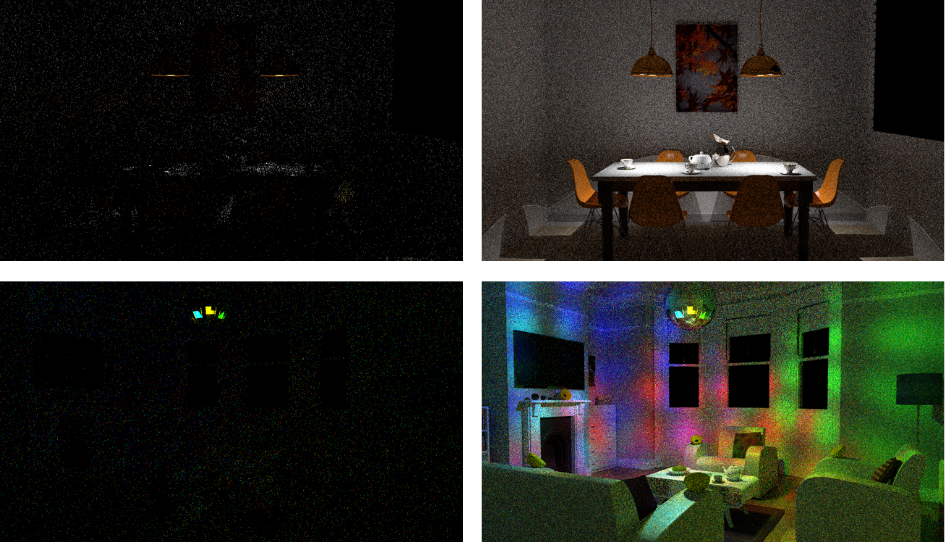
\includegraphics[width=1\linewidth]{img/ruppert_vs_rath.png}
        \caption{Porównanie path guidingu wykorzystującego rozkład kierunkowy (po lewej) i rozkład przestrzenny (po prawej)\footcite{Focal_Guiding}}
        \label{fig:enter-label}
    \end{figure}
\end{frame}

\section{Plan pracy}
\begin{frame}{Perspektywa poprawy}
\begin{itemize}
    \item Jako że funkcja wkładu punktu jest ciągła, można spróbować oszacować ją za pomocą mieszaniny rozkładów Gaussa.
    \item Potencjalnie może to poprawić obsługę efektów ogniskowych oraz zmniejszyć ilość potrzebnych próbek.
\end{itemize}
\begin{figure}
    \centering
    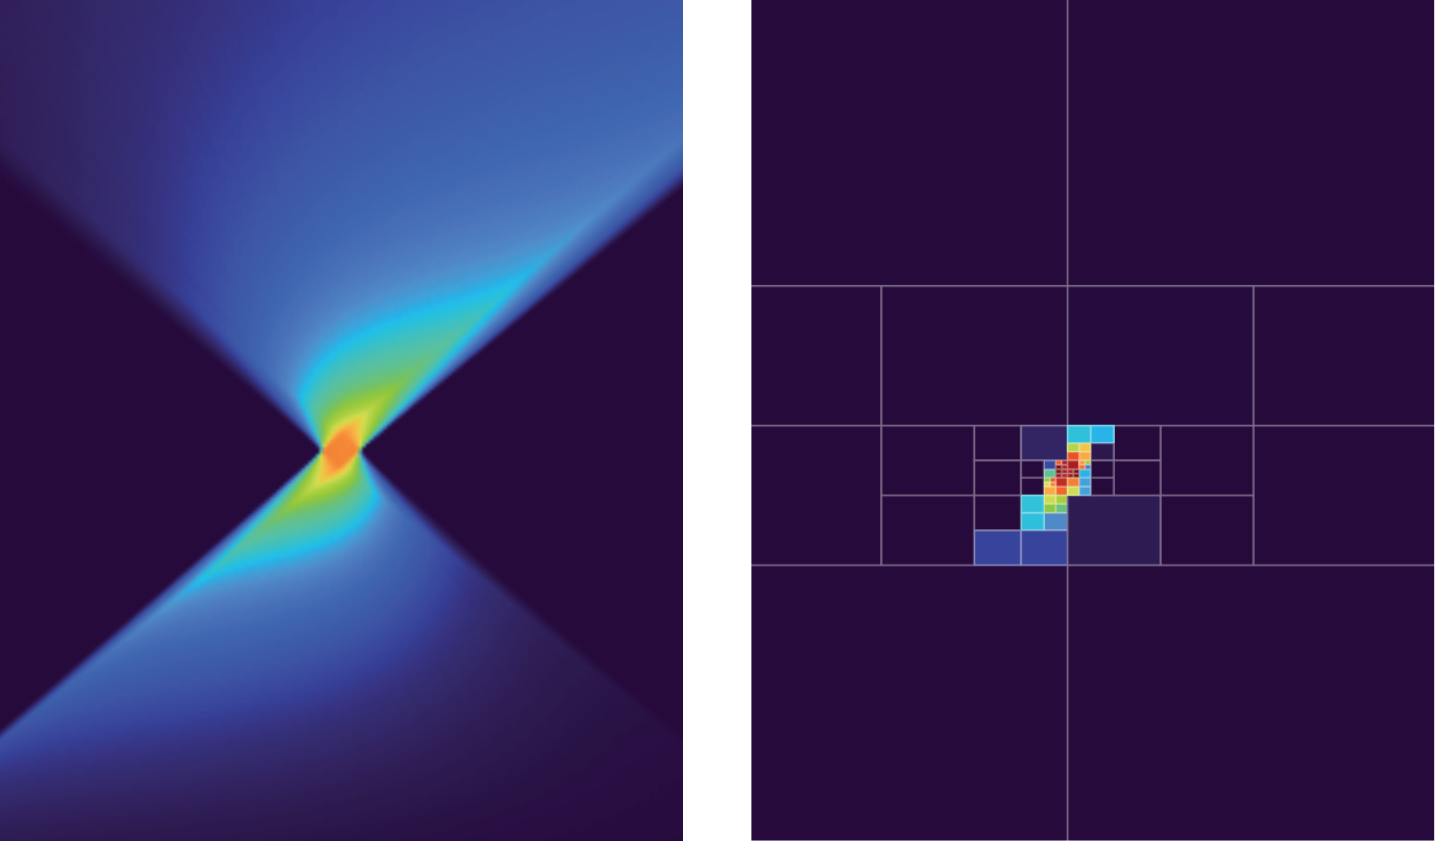
\includegraphics[width=0.5\linewidth]{img/descrite_vs_continuous.png}
    \caption{Ciągła i dyskretna reprezentacja funkcji wkładu punktu\footcite{Focal_Guiding}}
    \label{fig:enter-label}
\end{figure}
\end{frame}

\begin{frame}{Plan pracy}
    \begin{itemize}
        \item Stworzenie mieszaniny rozkładów Gaussa, która będzie szacować funkcję wkładu punktów.
        \item Zbieranie danych do dopasowania mieszaniny podczas każdej iteracji renderingu.
        \item Używanie dopasowanej do funkcji wkładu mieszaniny do prowadzenia kolejnych ścieżek w stronę ognisk.
    \end{itemize}
\end{frame}


\begin{frame}[allowframebreaks, noframenumbering]
    \frametitle{Bibliografia}
    \nocite{*}
    \printbibliography
\end{frame}
\end{document}
